\section{Uso de modelos matemáticos en economía}
\textit{Capítulo correspondiente en CORE ECON: \href{https://www.core-econ.org/the-economy/book/es/text/02.html}{Capítulo 2}}

\subsection{Función de producción y trampa de Malthus}
La trampa Malthusiana se refiere al periodo de estancamiento que se observa hasta el siglo XVIII. Se caracteriza por estar estancados el crecimiento poblacional y salarial.

\subsubsection{Modelo económico}
Sirve para
\begin{itemize}
    \item Capturar elementos fundamentales y los \hyperlink{trade-off}{trade-off} en los cuales se basan las decisiones
    \item Identificar situaciones de \hyperlink{equilibrio}{equilibrio}
    \item Incorporar relaciones entre los agentes que participan
    \item Explicar/predecir como evoluciona el sistema ante intervenciones
\end{itemize}

\subsubsection{Bases del modelo de Malthus}
\begin{itemize}
    \item Modelo de crecimiento de la población
    \begin{itemize}
        \item determinado por nivel de ingreso
        \item Ingreso de subsistencia es aquel que mantiene la población constante
    \end{itemize}
    \item Función de producción
    \begin{itemize}
        \item Determina la cantidad producida a partir de insumos
        \item Retorno decrecientes del trabajo: la productividad de cada trabajador adicional decrece a medida que aumenta la cantidad de trabajadores.
    \end{itemize}
\end{itemize}

\subsubsection{Función de producción}
Expresión gráfica o matemática que describe la cantidad de producto que puede generarse con cualquier cantidad. Viene dada por

\[Y = f(N)\]

donde $Y$ es la cantidad de unidades producidas, $f$ la función de producción y $N$ el número de trabajadores. En base a esta se puede definir la productividad promedio o productividad por trabajador como $w = \frac{Y}{N}$
\\

Una función de producción presenta retornos decrecientes cuando la productividad por trabajador va decreciendo a medida que aumenta el número de trabajadores. 

\begin{figure}[H]
    \centering
    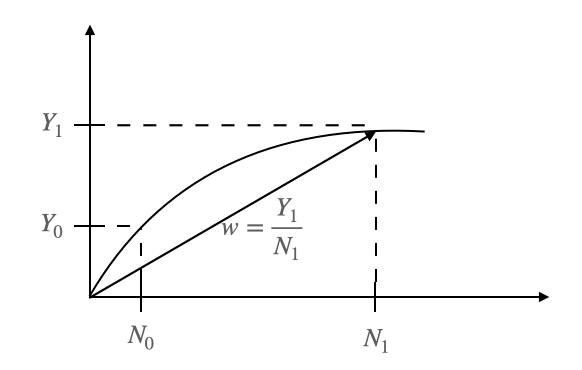
\includegraphics{Modulo_1/retornos_decrecientes.png}
    \caption{Visualización de los retornos decrecientes, al ser $\frac{Y_1}{N_1} < \frac{Y_0}{N_0}$}
\end{figure}

\subsubsection{Modelo de crecimiento poblacional} (depende del nivel de bienestar)
\\

En este modelo se representa el bienestar mediante el salario por trabajador, que a su vez se define como la producción por trabajador.

La tasa de crecimiento de la población es una función que depende del salario.
\\

Sea $w_s$ el salario de \hyperlink{subsistencia}{subsistencia} el valor donde se estabiliza la población, entonces si $w > w_s$ la población crece y si $w < w_s$ la población decrece. 
\\

Si $g(w) = \frac{N_t}{N_{t-1}}$ mide el crecimiento de la población, entonces $g(w_s) = 1$ y $w_t = \frac{Y_t}{N_t}$.

Donde el único salario en equilibrio es el de subsistencia que mantiene el crecimiento de la población estable. \[\frac{Y^*}{N^*} = w_s \implies N^*\cdot w_s = f(N^*)\]

\subsection{Innovación tecnológica}
Nuevas tecnologías causan que la productividad a un mismo número de trabajadores aumente, moviendo la cantidad de población del equilibrio.

Si se introducen tecnologías más rápido de lo que puede equilibrarse el sistema se da un crecimiento de los salarios y de la población, simultáneamente. \textit{(Justo esto es la revolución industrial, que permite el escape de la trampa Malthusiana)}

\subsection{Función de costos}
A la hora de escoger tecnologías es importante tener en cuenta su eficiencia y costos. La función de costos viene dada por
\[C(L, w) = w \cdot L + r\cdot K\]
Donde:
\begin{itemize}
    \item L = número de trabajadores
    \item w = salario de trabajadores
    \item r = precio de materiales
    \item K = cantidad de materiales
\end{itemize}


Si despejamos $K$ de la función de costos obtenemos la \textit{curva de isocostos}, esta representa todas las combinaciones que cuestan una cantidad total determinada. \textit{También conocido como: isocoste.}
\[K = \frac{C}{r} - \frac{w}{r}L\quad \quad \text{(C fijo)}\]


En un gráfico para poder determinar que tecnologías son más eficientes que otras hay que comparar la cantidad de insumos que debe utilizar, mientras menor sea la cantidad mejor es en comparación a las demás. En \href{https://www.core-econ.org/the-economy/book/es/text/02.html#qué-es-una-tecnolog}{este capítulo} del CORE se muestra como poder discernir entre 5 tecnologías competentes (Segundo sector con imágenes). 

\subsubsection{Cambio de tecnologías}
Cuando cambian los costos de los insumos, se tiene que algunas tecnologías podrían pasar a ser más baratas que otras. Esto conlleva que sea necesario cambiar de tecnología para minimizar los costos, la variación en costos de las tecnologías existentes se puede ver de manera gráfica dibujando las curvas de isocostos, y el cambio en ganancias por cambiar de tecnología es
\[\text{cambio en ganancias} = \text{cambio en ingresos} - \text{cambio en costos}\]
Donde, cambio en costos = $\text{costo}_{\text{final}} - \text{costo}_{\text{inicial}}$.
\newpage